% +------------------------------------------------------------------------+
% | CGAL Reference Manual:  qt_widget.tex
% +------------------------------------------------------------------------+
% | Using Qt_widget to visualize CGAL Objects
% | 
% |
% |
% | 12.12.2001  Radu Ursu
% | 

% +------------------------------------------------------------------------+

\newcommand{\qt}{{\em Qt}}      %QT abbreviation

\gdef\lciIfHtmlClassLinks{\lcFalse}
\gdef\lciIfHtmlRefLinks{\lcFalse}
\gdef\lciIfHtmlLinks{\lcFalse}


\begin{figure}[h]
\begin{ccTexOnly}
\begin{center}
\includegraphics{Qt_widget/triangulation.eps} 
\end{center}
\end{ccTexOnly}
\begin{ccHtmlOnly}
<CENTER>
<IMG BORDER=0 SRC="triangulation.gif"  ALIGN=center  ALT="A Nice Screen Shoot">
</CENTER>
\end{ccHtmlOnly}
\end{figure}

\qt\ is a {\sc Gui} toolkit\footnote{http://www.trolltech.com} for
cross-platform application development. 

% +-----------------------------------------------------+
\section{Introduction}

This chapter describes the \ccc{Qt_widget} package which provides
an interface between \cgal\  and the  {\sc Gui} toolkit \qt\ .
The \ccc{Qt_widget} package allows to build \qt\ 
applications  showing two dimensional \cgal\ objects 
and algorithms.

%In this chapter we describe a widget and some helper classes that
%allow to interact with two dimensional \cgal\ objects in \qt\/ based applications.

The atom of the \qt\ user interface is called a widget.
A widget receives mouse, keyboard and other 
events from the window system, and paints a representation of itself on the 
screen. Widgets are rectangular, and the different widgets
of an application  are sorted in a Z-order. Widgets
can have a parent widget and  children.
A widget is clipped by its parent and by the widgets in front of it. 


The most important class in the package
is the class \ccStyle{Qt_widget} which implements a widget
providing 
a drawing area and output stream operators for \cgal\ 
two dimensional objects.  \ccStyle{Qt_widget} also provides
zooming and panning functionalities.

The \ccStyle{Qt_widget} allows to attach {\em layers}. Layers usually
draw on the drawing area of the widget. Layers can be activated and
deactivated, and what you see in the drawing area is the overlay of
all attached activated layers. Layers can also be used for entering
input, and \cgal\ provides input \ccc{layers} for the two-dimensional
\cgal\ objects.

The package includes also the class \ccc{Qt_widget_standard_toolbar}
 providing a  standard toolbar for controlling the basic functionality
of the \ccStyle{Qt_widget}.

The following sections describe the main class as well as the helper classes
in more detail and give examples that can be taken as starting points for
new applications.


\noindent {\bf Remark:} The \ccStyle{Qt_widget} is distributed under
the {\sc Qpl}, which is Trolltech's open source license. For more details
on the {\sc Qpl} see \verb+http://www.trolltech.com/developer/licensing/qpl.html+.

\section{Qt\_widget}
\label{Qt_widget}

The class \ccStyle{Qt_widget} is derived from the class 
\ccStyle{QWidget} 
%\footnote{A widget is the atom of the user interface: It receives mouse, keyboard and other 
%events from the window system, and paints a representation of itself on the 
%screen. Every widget is rectangular, and they are sorted in a Z-order. A 
%widget is clipped by its parent and by the widgets in front of it.} 
which is the base class of all \qt\ user interface objects. 


The \ccStyle{Qt_widget} provides output operators for two dimensional \cgal\
objects. There are operators defined for output of: points, segments, 
lines, rays, circles, triangles, rectangles, polygons, conics,  and all type of
triangulations. Also some operators are defined to set
\ccStyle{Qt_widget}'s properties, like background and fill color, as
well as line width and point size.

As the following examples show, simple applications can be written
without the layers.

\subsection{Example: Hello Segment}
The first example draws a red segment on an orange background.
\ccIncludeExampleCode{Qt_widget/Examples/hellosegment.C}

We follow the \qt\ naming conventions for material properties, for
example, the {\tt CGAL::BackgroundColor} above.

All the drawing code should be put between \ccStyle{Qt\_Widget}'s lock() and
unlock() functions. See the manual reference pages of
\ccStyle{Qt\_widget}. Doing like this, the window will be updated only
once, when \ccStyle{Qt\_widget} finds the last unlock(). This way you
can avoid the window flickering.

This example has a severe drawback: when you resize the window it is
empty, as nothing is redrawn. This style of programs makes
only sense, if you quickly want to validate output of a geometric
computation. As in any event driven {\sc Gui} application,
 \qt\  provides a callback mecanism so
that the window system can update the drawing
whenever necessary. This is the topic of the next example.

\subsection{Example: Signals and Slots}

This example is slightly more involved and uses  the
signal/slots mecanism of \qt\ .

The main widget shows a
Delaunay triangulation. Every time the mouse button is pressed over 
the widget, a point is input  and inserted in the Delaunay
triangulation. The result of this insertion appears immediately.
Furthermore, the drawing is  updated every time the window is resized.


\ccIncludeExampleCode{Qt_widget/Examples/tutorial2.C}


\qt\ applications are event driven and respond to user interaction.
For example, when a user clicks on a menu item or on a toolbar button,
the application executes some codes. The programmer of an
application has to be able to relate events to the relevant code.
\qt\ provide for that the signals/slots mecanism:
\begin{description}
\item{\bf Signals.}
Each \qt\ widget declares a set of signals which, using the
keyword \ccc{emit}  can be  emitted by member functions 
under some circumstances. Signals are declared by using 
the keyword \ccc{signals:} just like an
access specifier in your class declaration.
\item {\bf Slots.}
A slot is just a member function declared under a public (or private)
slots section.
\item{\bf Connect.}
Signals and slots can be connected together using the method 
\ccc{connect}. This method needs to know four things: the object
that sends out the signal, the signal, 
the object to which belong the connected slot
and the slot connected to the signal.
For instance, the statement:
\begin{ccExampleCode}
connect(widget, SIGNAL(redraw_on_back()),
        this, SLOT(redraw_win()));
\end{ccExampleCode}

connects the signal \ccc{redraw_on_back()} of the widget \ccc{widget}
to the slot \ccc{redraw_win()} of the \ccc{QMainWindow} \ccc{his}.
Signals and slots can have any type of arguments, but a signal and a
slot connected together must have the same arguments types.
\end{description}

Every class that defines at least a signal or a slot must be derived
from the class \ccc{QObject} and must use the macro {\sc Q\_object}
inside the private section of its declaration. You also need to run
\ccc{moc}, the \emph{Meta Object Compiler} supplied with \qt\, on the
file that contains the class declaration.

\ccc{moc} is a pre-compiler that produces the \emph{meta object} code
of each class that uses the macro {\sc Q\_object}. This \emph{meta
  object} code is needed by the signal/slot mecanism. There are
several methods to compile the outputs of \ccc{moc}. In CGAL, we have
chosen to include the outputs of \ccc{moc} in a source files. See the
\qt\ documentation on \ccc{moc} for other possibilities.

The line \ccc{//moc_source_file : tutorial2.C} is for users that use
makefiles. This line tells to the \cgal\ makefile generator that
\ccc{tutorial2.C} should be the file that \ccc{moc} should be run on.

Let us come back to the control flow in the above example.
The main widget of the application is the widget \ccc{w}
of  class \ccc{My_window}.  The creator  of 
\ccc{My_window} triggers the creation of a \ccc{Qt_widget}
accessible through the pointer \ccc{widget}.
When  the mouse button is pressed in its drawing area,
the \ccc{Qt_widget} 
emits the signal  \ccc{s_mousePressEvent(QMouseEvent*)}
connected to the slot \ccc{mousePressEvent(QMouseEvent*)} of \ccc{My_window}.
This slot inserts the point in the Delaunay triangulation
and calls the method \ccc{redraw()} of \ccc{Qt_widget}.
The  \ccc{redraw()} method of \ccc{Qt_widget}
emits the signal \ccc{redraw_on_back()}. This signal is
connected to the slot \ccc{redraw_win()}
of  \ccc{My_window} which actually draws the triangulation.
Note that the  \ccc{Qt_widget}  emits the same signal
\ccc{redraw_on_back()} when the window is resized. Thus,
the signals/slots connection  ensures that the
triangulation is redrawn  each time the redrawing is needed.


\begin{ccAdvanced}
There are several ways to draw something with \ccc{Qt_widget}. One way
is to use the signals \ccc{redraw_on_back()}, \ccc{redraw_on_front()}.
This way you can bring your drawings before all or after all the
other drawings. An other option is to use the \ccc{QPainter} instance 
of \ccc{Qt_widget} that you can get calling \ccc{get_painter()}
method. The most recommended way is to use layers, that are described
in the next section.
\end{ccAdvanced}

Note that in that example, the \ccc{My_window} constructor calls
\ccc{new} to allocate a new \ccc{Qt_widget} object but \ccc{delete} is
never called to deallocate it. This does not mean that there is a
memory leak. It is in Qt's responsability to free widgets that have a
parent. In that example the \ccc{My_window} object is the parent of
\ccc{widget} and will deallocate it automatically at its destruction.

\section{Layers}
\label{Qt_widget_layers}
\subsection{Using Layers to Draw}

In the examples from the previous section the code for drawing on the
widget was in the \ccStyle{redraw_win()} function. As soon as the
applications are more involved it leads to a more modular design if
one delegates the drawing task to {\em layers}. For example, if the
application displays a Delaunay triangulation, the corresponding
Voronoi diagram, and at the same time highlights the nearest vertex to
the mouse coordinates, it makes sense to have three independent
layers. Besides better code, layers have the advantage that they can
be activated and deactivated at runtime. Finally, more modularity
means a higher potential for reuse.

A layer can be {\em attached} to a \ccc{Qt_widget}. The \ccc{redraw()}
member function of the \ccc{Qt_widget} calls
the method \ccc{Qt_widget_layer::draw()} of all attached layers, in the
order that they were attached. It is a very simple rule: the last layer
attached will be drawn on top.

Also a layer can be {\em activated} and {\em deactivated}. Only active
layers are drawn, and by default a layer is activated when it gets
attached.  Note that deactivating and activating do not influence the
order of layers. You can change the order only by attaching and
detaching it.


\cgal\ provides a base class so that users can write their own
layers. All the layers have to derive from this base class
\ccc{Qt_widget_layer} to have the functionality described.


\subsection{Example: Using a Layer to Draw}

\ccExample
\begin{ccExampleCode}
#include <CGAL/Cartesian.h>
#include <CGAL/Point_2.h>
#include <CGAL/Delaunay_triangulation_2.h>
#include <CGAL/IO/Qt_widget_Delaunay_triangulation_2.h>
#include <CGAL/IO/Qt_widget.h>
#include <CGAL/IO/Qt_widget_layer.h>
#include <qapplication.h>

typedef CGAL::Cartesian<double>             Rep;
typedef CGAL::Point_2<Rep>                  Point;
typedef CGAL::Delaunay_triangulation_2<Rep> Delaunay;

Delaunay dt;

class My_layer : public CGAL::Qt_widget_layer{
  void draw(){
    *widget << dt;
  }
};

class My_window : public CGAL::Qt_widget {
public:
  My_window(int x, int y)
  {
    resize(x,y);
    attach(&layer);
  };
private:
  //this method is called when the user presses the mouse
  void mousePressEvent(QMouseEvent *e)
  {
    Qt_widget::mousePressEvent(e);
    dt.insert(Point(x_real(e->x()), y_real(e->y())));
    redraw();
  }
  My_layer layer;
};

int main( int argc, char **argv )
{
    QApplication app( argc, argv );
    My_window *W = new My_window(400,400);
    app.setMainWidget(W);
    W->show();
    W->set_window(0, 400, 0, 400);
    return app.exec();
}
\end{ccExampleCode}

This example defines a class derived from
\ccStyle{Qt_widget_layer}. In the member function \ccStyle{draw()}
is the code for drawing the triangulation. In \ccStyle{My_Window}
class you need an instance of \ccStyle{My_Layer} and you will 
have to attach it, if you want to see what the layer draws on the
screen.

As you see, this example is very similar to the previous one, but
the code for drawing the triangulation is no longer in the
\ccStyle{redraw_win()} function, but in a layer.



\subsection{Using Layers to Build New Objects }
\label{Qt_widget_tools}

The main purpose of layers is to have more modular code for drawing on
the widget. Things are similar for handling input. In the previous
examples, input went through the \ccc{Qt_widget::mousePressedEvent()}
callback, which interpreted the input. In applications where you have
different kinds of input, e.g., segments and polygons in an
arrangement demo, this quickly leads to unreadable, difficult to maintain
code,  especially as typically more than one event callback is
involved. The proper way of decomposition, is delegation
of the event handling to a {\em layer}. 

A layer for \ccStyle{Qt_widget} receives all the events from
\ccStyle{Qt_widget} if it is active and can provide some functionality
like input objects for \ccStyle{Qt_widget}. Notice that the layers
receive events in the order they have been attached. Layers can have
internal state, because for entering complex objects it needs several
events. Therefore layers must have functions to initialize state when
they are activated and to clean up when they are deactivated.

\cgal\ provides some predefined input layers. You can have a lot of
layers attached that could be active in the same time. You have to
take care how you manage the events if you do not want to have
conflicts. A conflict is when two attached layers that are active need 
both the same event and getting and using it might not have such a
good effect in your application. For example the predefined layers that 
builds a new line and a new circle produce bad visual effects when are 
both active.

You can resolve conflicts by using \ccc{layers} exclusive. If you have 
several layers that can not be active at the same time without creating
conflicts, you can resolve that by letting the user not activate
more than one of those at a time.

\begin{ccAdvanced}
In all the \cgal\ demos that are provided, the layers are used with a
toolbar and buttons. To activate and deactivate a layer you have to
click one of the toolbar buttons. There are layers that need exclusive 
use. This is accomplished by grouping the buttons in one group, and
making that group exclusive. The group class is \ccc{QButtonGroup} that
comes with \qt\ .
\end{ccAdvanced}

We first show how to use layers and then how they work.

\subsection{Example: How to Use a Layer}

In the previous section, you could insert new points in the
triangulation by clicking on the widget. This example shows how
the same can be achieved with the help of a layer.

We attach the predefined layer \ccc{Qt_widget_get_point} to the widget,
and connect the signal emitted by the widget to the function that
handles the input.  When the user clicks with the left mouse button,
the layer creates a point and passes it to the widget. The widget then
emits a signal that gets passed to the connected slot
\ccc{My_Window::get_new_object(CGAL::Object)}.

\ccIncludeExampleCode{Qt_widget/Examples/layer.C}

The \ccStyle{Qt_widget} forwards all events that it receives to the
attached and active layers. If a layer is attached but not active, it
does not get the events. It is put in a passive state. Activating and
deactivating the layer does not mean that the object is destructed.

\subsection{Example: How Layers Work}

The following is an example of a \ccc{layer} that creates \cgal\ points when
the user clicks the left mouse button over the widget. 
 
\begin{ccExampleCode}
#include <CGAL/IO/Qt_widget.h>
#include <CGAL/IO/Qt_widget_layer.h>
#include <qcursor.h>

#ifndef CGAL_QT_WIDGET_GET_POINT_BUTTON
#define CGAL_QT_WIDGET_GET_POINT_BUTTON Qt::LeftButton
#endif

namespace CGAL {
template <class R>
class Qt_widget_get_point : public Qt_widget_layer
{
public:
  typedef typename R::Point_2   Point;
  typedef typename R::FT        FT;
  
  Qt_widget_get_point(const QCursor c=QCursor(Qt::crossCursor),
                      QObject* parent = 0, const char* name = 0) :
    Qt_widget_layer(parent, name), cursor(c) {};
  
private:
  bool is_pure(Qt::ButtonState s){
    if((s & Qt::ControlButton) ||
       (s & Qt::ShiftButton) ||
       (s & Qt::AltButton))
      return 0;
    else
      return 1;
  }
  void mousePressEvent(QMouseEvent *e)
  {
    if(e->button() == CGAL_QT_WIDGET_GET_POINT_BUTTON
       && is_pure(e->state()))
    {
      FT x, y;
      widget->x_real(e->x(), x);
      widget->y_real(e->y(), y);
      widget->new_object(make_object(Point(x, y)));
    }
  };
  void activating()
  {
    oldcursor = widget->cursor();
    widget->setCursor(cursor);
  };
  
  void deactivating()
  {
    widget->setCursor(oldcursor);
  };

  QCursor cursor;
  QCursor oldcursor;
};
} // namespace CGAL
\end{ccExampleCode}

The \ccc{Qt_widget} forwards mouse and keyboard events to the attached layer.
In the above example only the \ccc{mousePressEvent} member function is overloaded.

Tools that create new \cgal\ objects, must call the member 
function \ccStyle{Qt_widget::new_object(CGAL::Object)}. The
\ccStyle{Qt_widget} then emits the signal
\ccStyle{new_cgal_object(CGAL::Object)}. This signal can be routed to
any slot of other object accepting a \ccc{CGAL::Object}, with the
following connect statement:
\begin{ccExampleCode}
connect(qt_widget_ptr, SIGNAL(new_cgal_object(CGAL::Object)), 
        any_other_object_ptr, SLOT(any_other_slot(CGAL::Object)));
\end{ccExampleCode}

The first argument must be a pointer to an instance of \ccc{Qt_widget}.
In the example we connect it to \ccc{MyWindow::get_new_object(CGAL::Object)}.

\section{The Standard Toolbar}
\label{Qt_widget_standard_toolbar}

The \ccStyle{Qt\_widget} allows to zoom and pan. This functionality is 
accessible through the class \ccStyle{Qt_widget_standard_toolbar}. The 
example further down shows how to use it in your application.

\begin{figure}[h]
\begin{ccTexOnly}
\begin{center}
\includegraphics{Qt_widget/standard_toolbar.eps} 
\end{center}
\end{ccTexOnly}
\begin{ccHtmlOnly}
<CENTER>
<IMG BORDER=0 SRC="standard_toolbar.gif"  ALIGN=center  ALT="The
standard toolbar">
</CENTER>
\end{ccHtmlOnly}
\end{figure}

\newcounter{bean}
The functionality of the toolbar is as follows from the left to right:
\begin{description}
%       {Button---\Roman{bean}}{\usecounter{bean}\setlength{\rightmargin}{\leftmargin}}
         \item[History back:] Go back into the transformation history
        \item[History forth:] Go forth into the transformation history
        \item[Zoom In:] The scaling factor is multiplied by two,
keeping the same center.
        \item[Zoom Out:] The scaling factor is divided by two, keeping
the same center.
       \item[Point tool:] Deactivate the layers corresponding to the
three following buttons which form an exclusive group
        \item[Focus on Point:] Lets you choose the center of the
region where you want to focus.
        \item[Focus on the Region:] The area in the rectangle that you selected will be magnified to best fit in the window.
        \item[Hand Tool:] Used for translate. Click to select the
first point of translation and drag to select the second point.
        \item[Mouse Coordinates Layer:] Mouse coordinates are
displayed on the status bar of your window.  You can deactivate this
layer if you click on it. To activate it again just click one more time.
\end{description}



\ccExample
\ccIncludeExampleCode{Qt_widget/Examples/standard_toolbar.C}

This example generates 100 points and inserts them in a Delaunay
triangulation. Using the standard toolbar you can zoom in, zoom out,
translate.

\section{The Help Window}
\label{The Help Window}

We provide a class in the \ccc{Qt_widget} library that was taken from
an example of \ccc{Qt} and adapted to our needs. This class has the
functionality of a rich text browser with hypertext navigation. You
can also PRINT, GO BACK, GO FORWARD or GO HOME. This class is called
\ccStyle{Qt_help_window} and you can use it to display hypertext support
in your application. It is used in a lot of demos provided in the
distribution.

\ccExample
\begin{ccExampleCode}
    #include <CGAL/IO/Qt_help_window.h>
        ....
    QString home = "help/index.html";
    Qt_help_window *help = new Qt_help_window(home, ".", 0, "help viewer");
    help->resize(400, 400);
    help->setCaption("Demo HowTo");
    help->show();
\end{ccExampleCode}

\section{Some Predefined Icons}
\label{The predefined icons}

\cgal\ provides some icons defined in some header files. The icons are
pixmaps, having the extension \ccc{.xpm}. Their location is \ccc{/include/CGAL/IO/pixmaps}.

To use a pixmap in your code you have to include the right file, and
to know the names of the pixmaps. The names of the pixmaps are
composed of two parts, the name of the file and the tag xpm. So for
example the arrow pixmap has the name \ccStyle{arrow\_xpm}, the line
pixmap has the name \ccStyle{line\_xpm}, and so on. There are also 
pixmaps files that contain small icons. The name of the smaller 
pixmaps contain a \ccc{small} at the middle of it like \ccStyle{point_small_xpm}.
In the tutorials and demos, almost all the pixmaps are used for the 
toolbar buttons, like this:

\ccExample
\begin{ccExampleCode}
    
    #include <CGAL/IO/pixmaps/point.xpm>
    
    QIconSet set(QPixmap( (const char**)point_small_xpm ),
                  QPixmap( (const char**)point_xpm ));

    QToolButton *point_button;
    point_button = new QToolButton(toolbar_ptr, "POINT INPUT BUTTON");
    point_button->setIconSet(set);
    point_button->setTextLabel("POINT INPUT LAYER");

\end{ccExampleCode}



\section{What Shall I Use?}

The previous sections presented different ways of writing \qt\ based 
applications. We recommend to use layers for the drawing task and for
input handling, even if you write tiny applications, because in general
they grow over time. Layers are a little bit more overhead, but 
it pays off in the long run, as you then do not have to completely
reorganize your code, to add layers. 

% +-----------------------------------------------------+
% EOF







